\section{Analyse und Auswertung}

\begin{frame}{Benchmark WebServer}
	\begin{figure}
		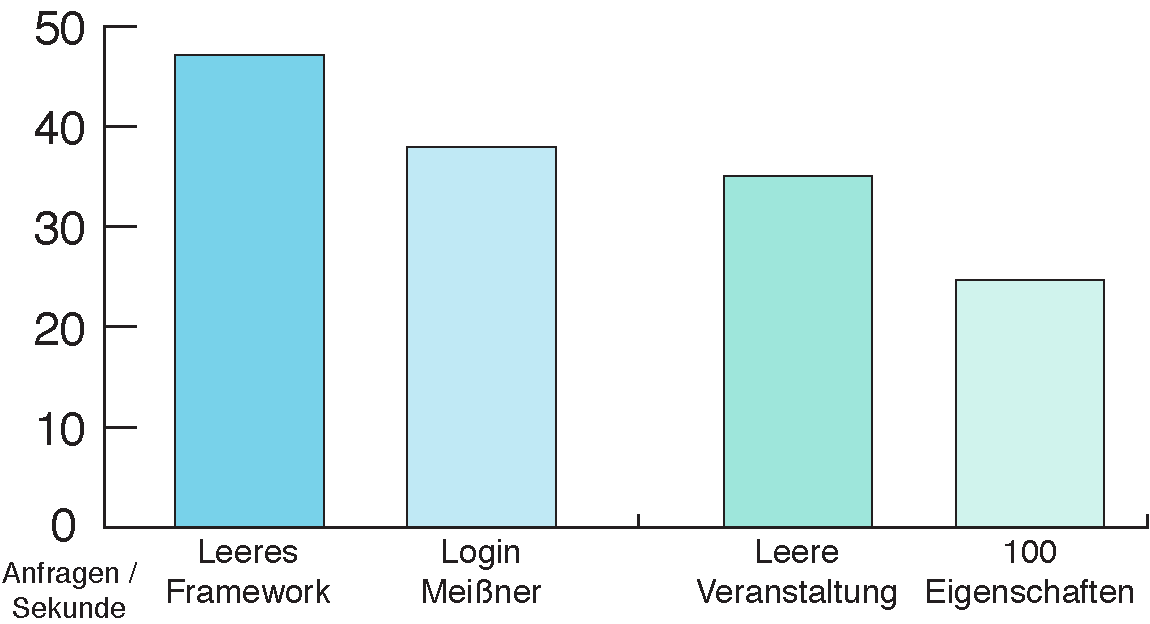
\includegraphics[width=0.7\textwidth]{fig/statistiken_ab.pdf}
	\end{figure}
	\begin{itemize}
		\item Apache Bench: 1000 Verbindungen, immer 10 gleichzeitig
		\item Praxis: Weniger Anfragen nötig durch Offline Cache
	\end{itemize}
\end{frame}

\begin{frame}{WebSocket Server}{Netzwerkauslastung}
	\begin{itemize}
		\item WebSockets: nur 2 Bytes Overhead!
		\item Normale HTTP Anfragen (Polling o.Ä.): 700-800 Bytes Overhead
		\item Besonders relevant bei hoher Anzahl von Clients\pause, bspw. 1.000 Clients:
		\item[]
	\end{itemize}

	\renewcommand{\arraystretch}{1.4}
	\centering
	\begin{tabular}{c|c|c}
		\textbf{Polling} & \textbf{WebSockets} & Einheit\\
		\hline
		800.000 &  2.000 & $\frac{Bytes}{Sekunde}$\\
		6.400.000 &  16.000 & $\frac{Bits}{Sekunde}$\\
		{\color{red}\textbf{6,104} :-(} & {\color{blue}\textbf{0,015} :-)} & $\frac{MBit}{Sekunde}$\\
	\end{tabular}

	\begin{itemize}
		\item[]
		\item[$\Rightarrow$] {\color{red}\textbf{Ersparnis von 400\% Traffic}}
	\end{itemize}
\end{frame}

\begin{frame}{Besonderheiten der Webanwendung}
	\begin{itemize}
		\item Eigenständig lauffähige Webanwendung
		\item Echtzeitaktualisierung
		\item Unterstützung von mobilen Geräten
		\begin{itemize}
			\item Offline Cache!
		\end{itemize}
		\item Automatisches Installationsskript für debianbasierte Systeme
		\item Für die Nutzung im Freien ausgelegt
		\item Modular aufgebaut
		\item Ähnliche Produkte kosten mehrere hundert Dollar und sind meistens nur als Erweiterung für WordPress verfügbar
	\end{itemize}
\end{frame}